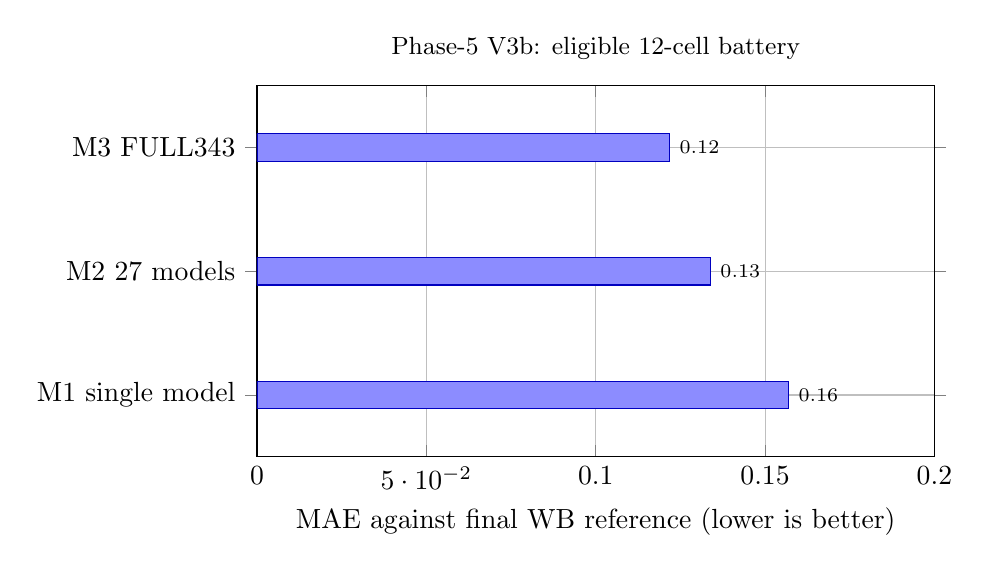
\begin{tikzpicture}
\begin{axis}[
  xbar, width=0.84\linewidth, height=63mm,
  xmin=0, xmax=0.20, xlabel={MAE against final WB reference (lower is better)},
  symbolic y coords={M3 FULL343,M2 27 models,M1 single model},
  ytick=data, y dir=reverse,
  nodes near coords, nodes near coords align={horizontal},
  every node near coord/.append style={font=\scriptsize},
  xtick={0,0.05,0.10,0.15,0.20},grid=major,
  enlarge y limits=0.25, bar width=10pt,
  title={Phase-5 V3b: eligible 12-cell battery},
  title style={font=\small},
]
\addplot[fill=blue!45,draw=blue!75!black] coordinates {
(0.157015315,M1 single model)
(0.133950984,M2 27 models)
(0.121889894,M3 FULL343)
};
\end{axis}
\end{tikzpicture}
